\documentclass[10pt,a4paper]{book}
\usepackage{subfiles}
\usepackage{dgnc}
\graphicspath{ {./imag/} }

% modificamos el pi� de p�gina para las versiones preliminares
\fancyfoot[RE,LO]{\small{versi�n 0.59 - p�g.\thepage}}

% marca de agua que diga que esto est� en construcci�n
%\usepackage[printwatermark]{xwatermark}
%\newwatermark[allpages,color=gray!50,angle=45,scale=3,xpos=0,ypos=0]{EN CONSTRUCCION}
\usepackage{draftwatermark}
\SetWatermarkText{EN CONSTRUCCION}
\SetWatermarkScale{0.5}
%\SetWatermarkColor[gray]{0.5}
%\SetWatermarkFontSize{2cm}
%\SetWatermarkAngle{30}
\SetWatermarkLightness{0.95}

% _____________________________________________________________________________ Car�tula
\begin{document}

\frontmatter
	\thispagestyle{cover}
	
	\title{Lanzadores Espaciales}
	\author{Augusto Zumarraga, ...}
	\date{Abril de 2024}
	%\maketitle
	
%	\newgeometry and \restoregeometry
	
	\pagenumbering{gobble}
	
	\hspace{-4.45cm}
		\begin{minipage}[t]{\paperwidth}
			\centering
			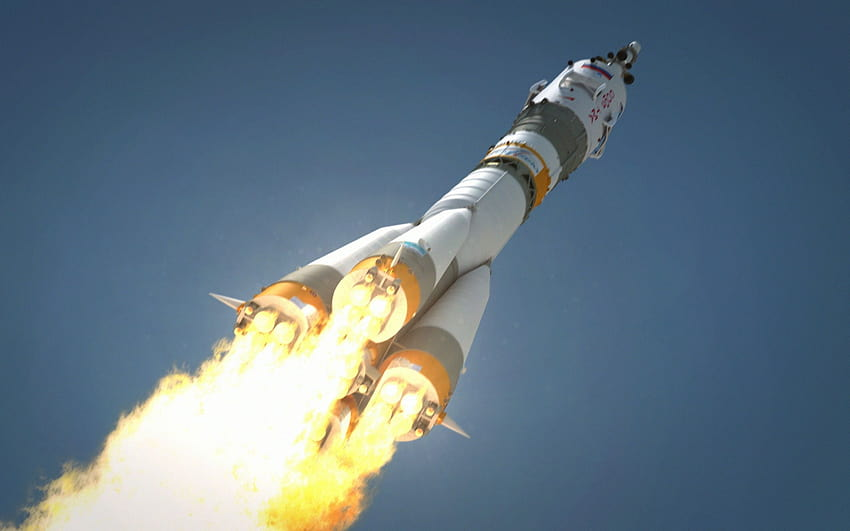
\includegraphics[width=\linewidth]{art/soyuz-3} 
		\end{minipage}
 
		\hspace*{2cm}
		\begin{flushright}
			{\fontsize{40}{50}\selectfont
				\textbf{\textsl{Lanzadores Espaciales}}\\
			}
			{
			\Huge\textit{Ingenier�a Aeroespacial - Edici�n 2024}
			}
			
			\vspace{1cm}
			
			\Large Augusto Zumarraga
		\end{flushright}

\begin{sloppypar}

% _____________________________________________________________________________ Indice
\tableofcontents

%	\chapter{Prefacio}
%	En este trabajo se persiguen dos objetivos principales: 
%	
%	\begin{itemize}[leftmargin=3cm]
%		\item plantear un paradigma unificado para el an�lisis din�mico, independientemente de la naturaleza f�sica del proceso analizado
%		\item presentar enfoques para construir modelos din�micos de estructuras y veh�culos aeroespaciales
%	\end{itemize}
%
%	Adem�s de manejar el c�lculo diferencial es fundamental para comprender los conceptos aqu� presentados dominar algunos aspectos b�sicos del �lgebra lineal tales como producto matricial, inversa y traspuesta de una matriz, y las propiedades caracter�sticas de matrices cuadradas (autovalores y autovectores).
%	\bigskip
%	
%	En el primer cap�tulo se plantea un enfoque amplio para sistematizar el an�lisis de los procesos din�micos recurriendo al modelo de estados y el an�lisis de equilibrio y estabilidad en el espacio de estados. 
%	A partir de esto se plantea la linealizaci�n del modelo para poder luego describir el comportamiento de forma universal a partir de modos naturales caracterizados por autovalores y autovectores de la matriz din�mica.
%	
%	Para este cap�tulo resultan fundamentales los conceptos de campo vectorial, serie de Taylor y transformada de Laplace.
%	\bigskip
%	
%	En el segundo cap�tulo se plantea el modelado de perturbaciones determin�sticas y el an�lisis de respuesta din�mica en el dominio del tiempo.
%	
%	Se Introduce la matriz de transferencia para el an�lisis de respuesta a perturbaciones determin�sticas, a partir de lo cual presentamos luego el an�lisis en frecuencia para perturbaciones peri�dicas, y con este el an�lisis espectral para perturbaciones aleatorias.
%	
	
% _____________________________________________________________________________ Cap�tulo 1
\mainmatter
\pagestyle{fancy}

%	\setlength{\parindent}{0cm} % Default is 15pt.
	%	\hangindent=3cm %This paragraph has an extra indentation at the left.
	% \setlength{\parskip}{4mm plus2mm minus2mm}
	
	\chapter{Trayectoria}
		\begin{center}
			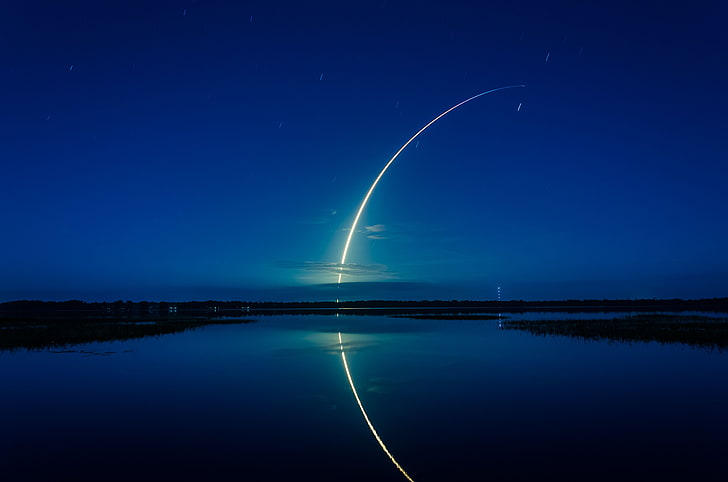
\includegraphics[width=1.02\linewidth]{art/trajectory-2}
		\end{center}
		\section{Introducci�n}
		\subfile{intro}
		\section{Trayectoria}
		\subfile{trayectoria}

%		\section{Modelos}
%		\subfile{modelado}
%		\subfile{estados}
%		\subfile{liapunov}
%		\section{Modelos Lineales}
%		\subfile{lineales}
%		\subfile{modos}
%		\subfile{solucion}

	\chapter{Din�mica}
		\begin{center}
			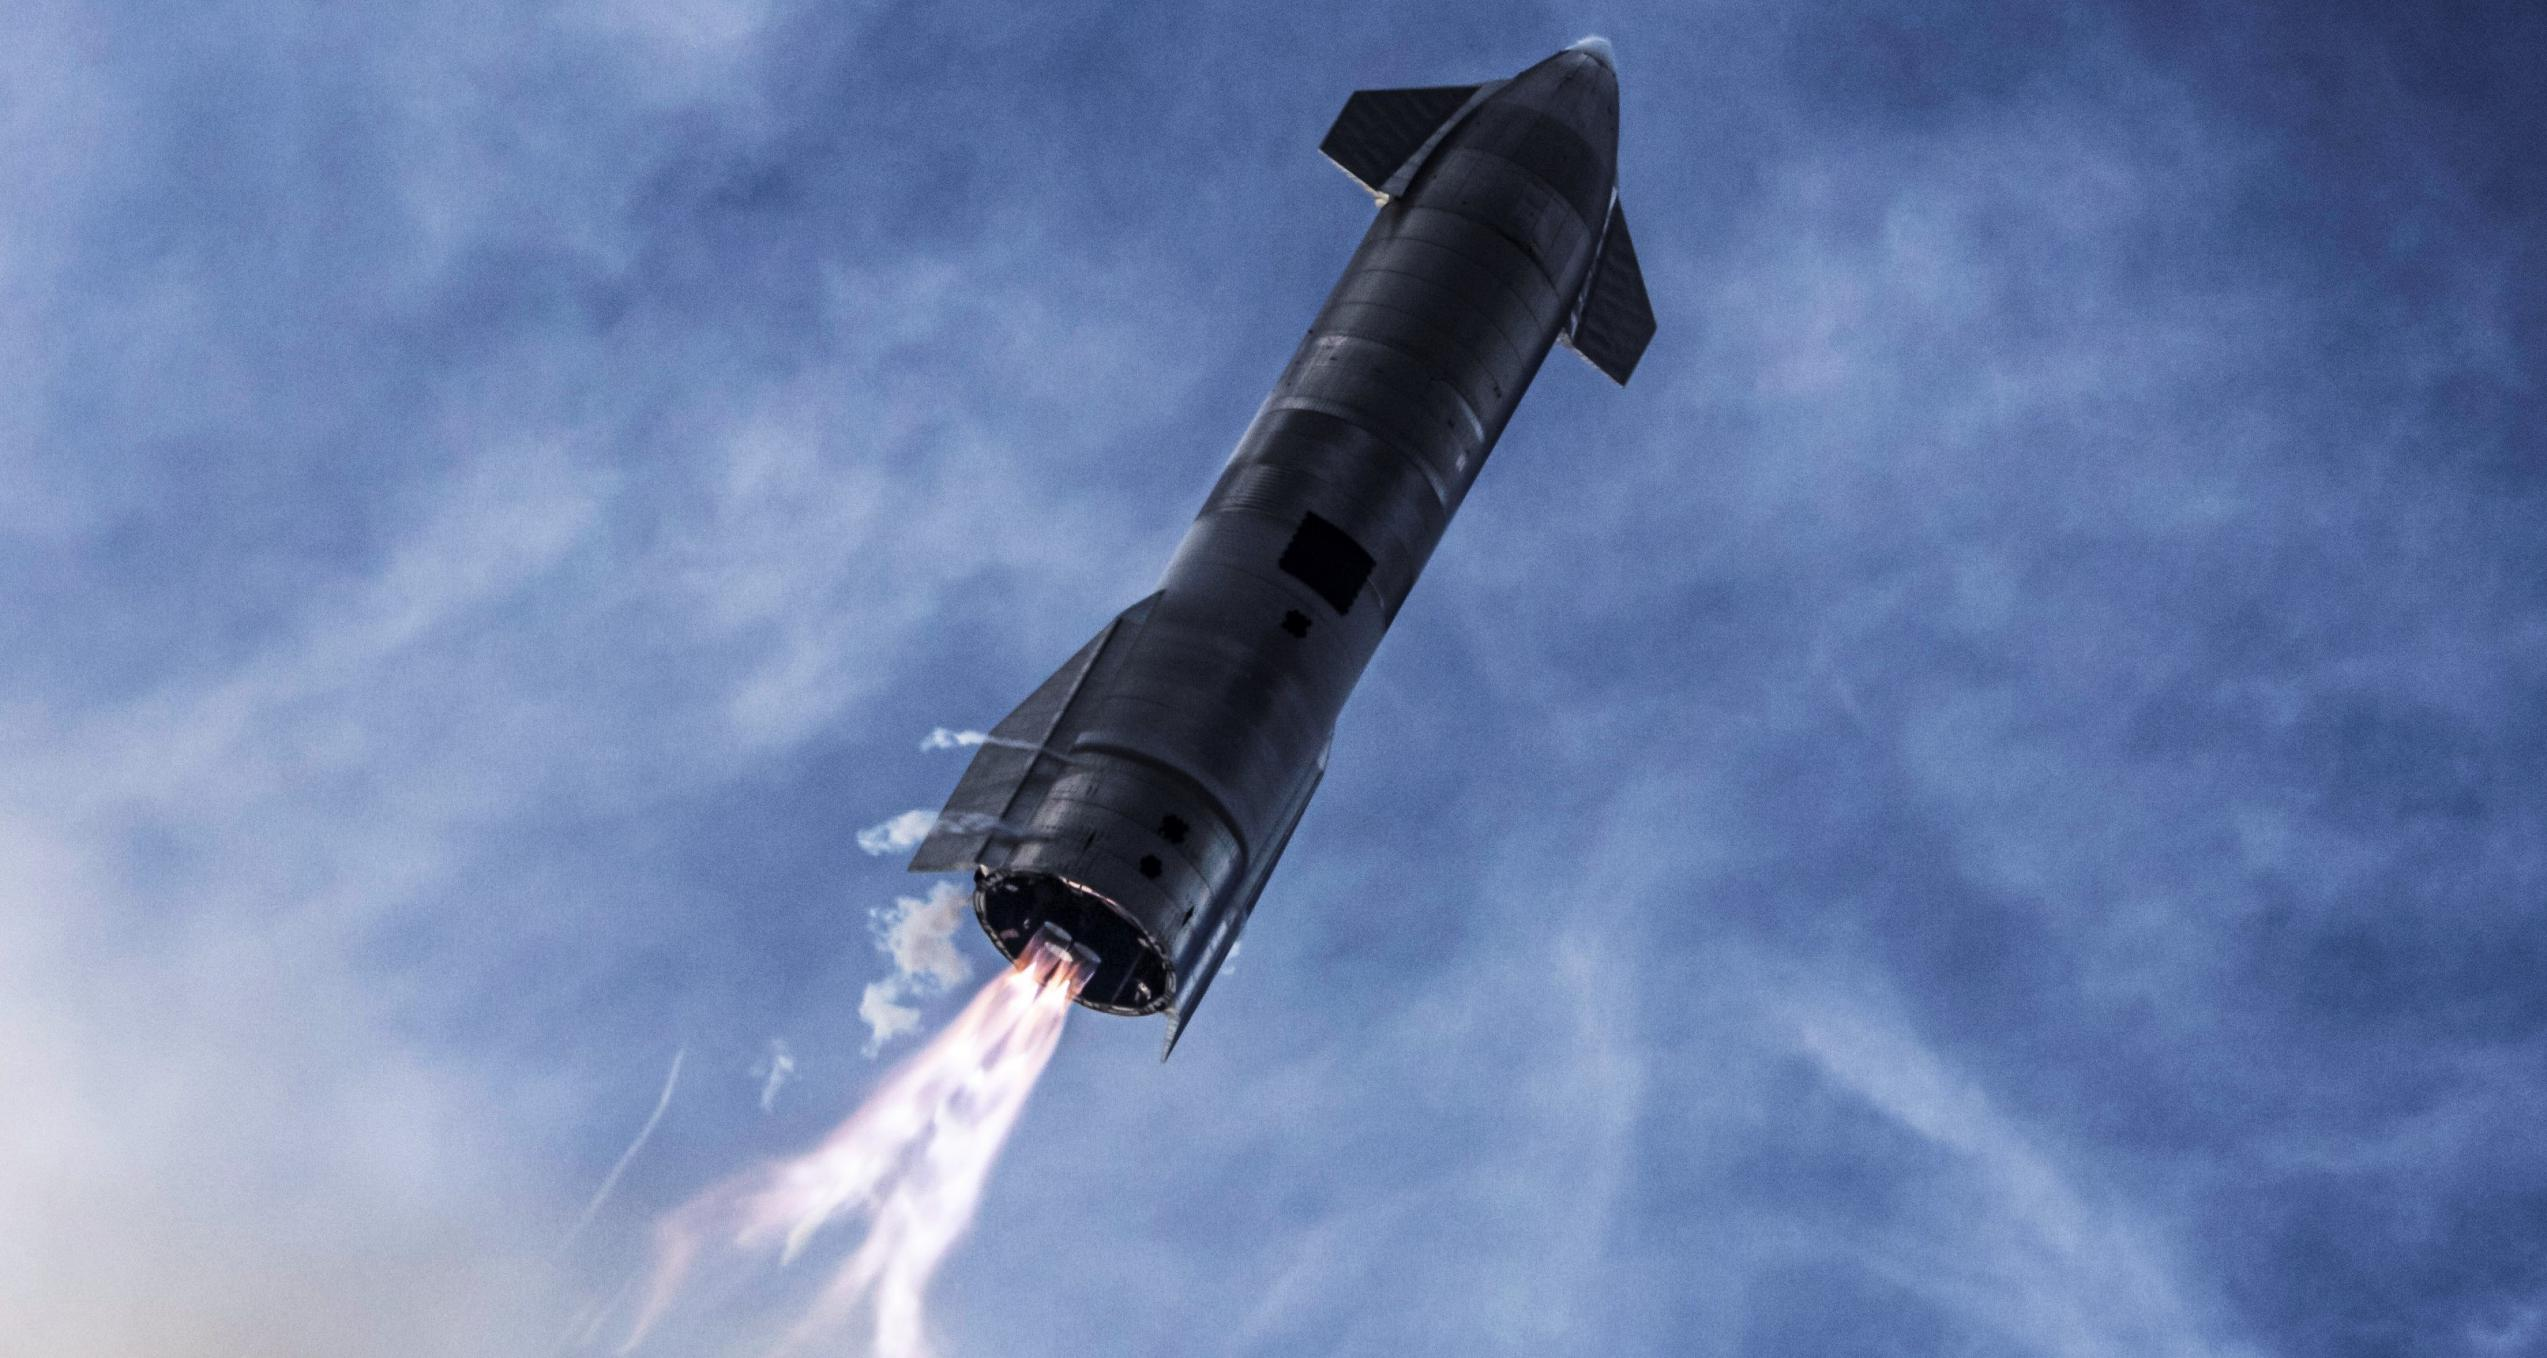
\includegraphics[width=1.02\linewidth]{art/starship-attitude}
		\end{center}
 		\section{Modelo de cuerpo r�gido}
		\subfile{rigido}
 		\section{Modelo estructural}
		\subfile{estructural}
 		\section{Modelo aeroel�stico}
		\subfile{elastico}
 		\section{C�mputos}
		\subfile{computos}
 		\section{Simulaci�n}
		\subfile{nav-sim}
		\subfile{elastic-sim}

	\chapter{Control de Vuelo}
		\begin{center}
			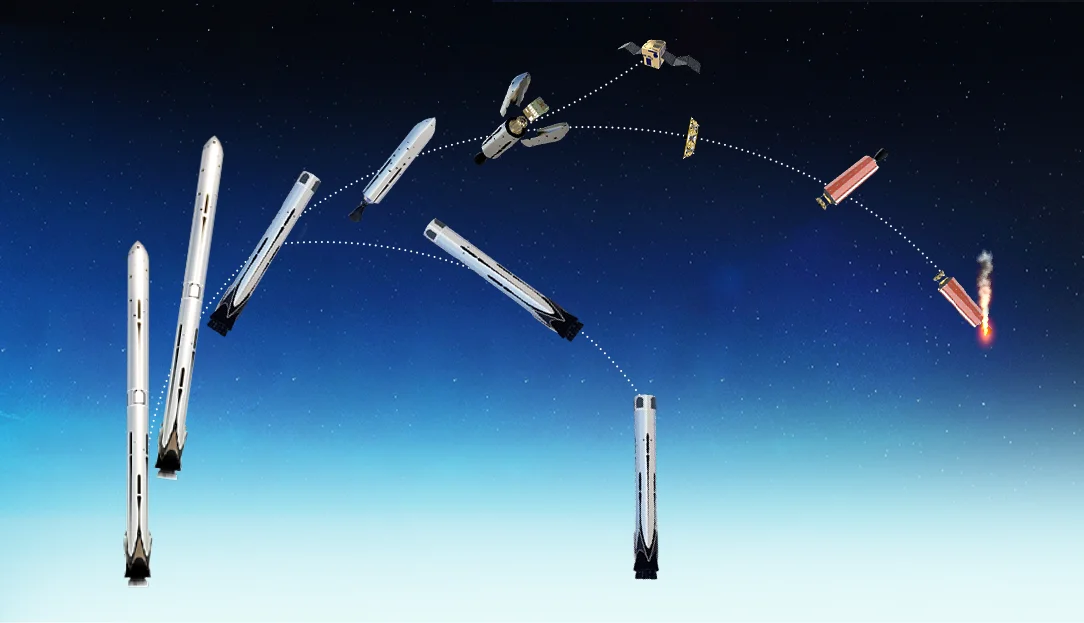
\includegraphics[width=1.02\linewidth]{art/falcon-staging}
		\end{center}
		\section{Guiado}
		\subfile{guiado}
 		\section{Control}
		\subfile{control}
		

	\appendix
	\chapter{Ap�ndices}
		\section{Aerodin�mica}
		\subfile{aero}\label{apnd:aero}
		\pagebreak
		\section{Interpolaci�n}
		\subfile{bicubic}\label{apnd:spline}
		%\subfile{turbulencia}\label{apnd:turbulencia}
		%\subfile{aeroelasticidad}\label{apnd:aeroelasticidad}

\backmatter
	
	\listoffigures
	%\listoftables

	\bibliographystyle{alpha}
	\bibliography{dgnc_biblio}{}


\end{sloppypar}
\end{document}
